%% LyX 2.2.3 created this file.  For more info, see http://www.lyx.org/.
%% Do not edit unless you really know what you are doing.
\documentclass[11pt,french,english]{article}
\usepackage[T1]{fontenc}
\usepackage[utf8]{inputenc}
\usepackage{amssymb}
\usepackage{amsmath}
\usepackage{ulem}
\usepackage{url}
\usepackage{graphicx}
\usepackage{enumitem}
\usepackage{bm}


\makeatletter

%%%%%%%%%%%%%%%%%%%%%%%%%%%%%% LyX specific LaTeX commands.
\providecommand{\LyX}{L\kern-.1667em\lower.25em\hbox{Y}\kern-.125emX\@}

\makeatother

\usepackage{lmodern}
\usepackage[english]{babel}
\makeatletter
\addto\extrasfrench{%
   \providecommand{\og}{\leavevmode\flqq~}%
   \providecommand{\fg}{\ifdim\lastskip>\z@\unskip\fi~\frqq}%
}

\makeatother
 
\usepackage{etoolbox}
\newcommand{\points}[2]{\iftoggle{undergrad}{{\color{red}[#1 points]}}{{\color{red}[#2 points]}}}
\newcommand{\enfr}[2]{\iftoggle{french}{#2}{#1}}
\newcommand{\instruct}[1]{\iftoggle{final}{}{#1}}
\newcommand{\proftitle}[2]{\iftoggle{undergrad}{#1}{#2}}
% \newcommand{\question}[1]{\\ \textbf{Question.} #1}

\providecommand{\LyX}{L\kern-.1667em\lower.25em\hbox{Y}\kern-.125emX\@}

\makeatother

\usepackage{lmodern}
\usepackage[english]{babel}
\makeatletter
\addto\extrasfrench{%
   \providecommand{\og}{\leavevmode\flqq~}%
   \providecommand{\fg}{\ifdim\lastskip>\z@\unskip\fi~\frqq}%
}

\makeatother



\usepackage[colorinlistoftodos]{todonotes}

\usepackage{todonotes}
\newcommand{\ioannis}[1]{\todo[inline,color=green!40,caption={}]{{\it Ioannis:~}#1}}
\newcommand{\guillaume}[1]{\todo[inline,color=blue!40,caption={}]{{\it Guillaume:~}#1}}

\newcommand{\gradpoints}[1]{\textcolor{red}{Graduates #1 pts}}
\newcommand{\undergradpoints}[1]{\textcolor{orange}{Undergraduates #1 pts}}




% Switch this to false to hide answers
\iftrue
\newcommand{\answer}[1]{\\ \textbf{Answer.} #1 }
\else 
\newcommand{\answer}[1]{}
\fi

\usepackage[colorlinks=true]{hyperref}

\newcommand{\blue}[1]{{\color{blue}#1}}
\newcommand{\w}{\mathbf{w}}
\newcommand{\x}{\mathbf{x}}
\newcommand{\ith}[1]{^{(#1)}}
%%%%%%%%% STUDENTS CHANGE THIS

\providetoggle{undergrad}
\settoggle{undergrad}{true}     %%% "true" if 3395 or "false" if 6390

\providetoggle{french}
\settoggle{french}{true}        %%% "true" if french or "false" if english

\providetoggle{final}            
\settoggle{final}{false}        %%% "true" for your final homework submission (removes instructions)

%%%%%%%%%%%%%%%%%%%%% ^^^^^


\usepackage[colorinlistoftodos]{todonotes}

\usepackage{todonotes}
\newcommand{\ioannis}[1]{\todo[inline,color=green!40,caption={}]{{\it Ioannis:~}#1}}
\newcommand{\guillaume}[1]{\todo[inline,color=blue!40,caption={}]{{\it Guillaume:~}#1}}

\newcommand{\gradpoints}[1]{\textcolor{red}{Graduates #1 pts}}
\newcommand{\undergradpoints}[1]{\textcolor{orange}{Undergraduates #1 pts}}


\newcommand{\french}[1]{ {\color{blue} #1} }


% toggle between grad and undergrad version
\usepackage{etoolbox}
\providetoggle{undergrad}
\settoggle{undergrad}{true}
\providetoggle{grad}
\settoggle{grad}{false}
%%%
% you can use e.g. \iftoggle{undergrad}{write something only in the undergrad version}{this will go only in the grad version}
%

% set points for undergrads and grads using one command:
\newcommand{\points}[2]{\iftoggle{undergrad}{{\color{red}[#1 points]}}{\color{red}[#1 points]}}
% usage: if the question is worth 5 points for undergrads and 3 for grads type
% \points{5}{3}

\usepackage[colorlinks=true]{hyperref}

\newcommand{\blue}[1]{{\color{blue}#1}}
\newcommand{\ith}[1]{^{(#1)}}

\renewcommand{\vec}[1]{{\bf #1}}
\newcommand{\mat}[1]{{\bf #1}}
\newcommand{\ten}[1]{\mat{\ensuremath{\boldsymbol{\mathcal{#1}}}}}
\newcommand{\mats}[1]{\ensuremath{\mathbf{\boldsymbol{#1}}}}
\newcommand{\vecs}[1]{\ensuremath{\mathbf{\boldsymbol{#1}}}}


\newcommand{\loss}{\ell}

\newcommand{\sigmoid}{\sigma}
\providecommand{\alert}[1]{{\color{MyRed}#1}}


\newcommand{\x}{\vec{x}}
\newcommand{\y}{\vec{y}}
\newcommand{\z}{\vec{z}}
\renewcommand{\u}{\vec{u}}
\renewcommand{\v}{\vec{v}}
\newcommand{\vmu}{\vecs{\mu}}
\newcommand{\w}{\vec{w}}
\newcommand{\X}{\mat{X}}
\newcommand{\Y}{\mat{Y}}
\newcommand{\W}{\mat{W}}
\newcommand{\K}{\mat{K}}
\newcommand{\I}{\mat{I}}
\newcommand{\M}{\mat{M}}
\newcommand{\U}{\mat{U}}
\newcommand{\D}{\mat{D}}
\newcommand{\A}{\mat{A}}
\newcommand{\B}{\mat{B}}
\renewcommand{\H}{\mat{H}}
\renewcommand{\S}{\mat{S}}
\renewcommand{\b}{\vec{b}}
\renewcommand{\a}{\vec{a}}
\newcommand{\MPhi}{\mats{\Phi}}
\newcommand{\Mphi}{\mats{\Phi}}

\DeclareMathOperator*{\Prob}{\mathbb{P}}
\DeclareMathOperator*{\Esp}{\mathbb{E}}
\newcommand{\ind}{\mathrm{I}}

%% Tensor stuff
\newcommand{\T}{\ten{T}}
\newcommand{\ttm}[1]{\times_{#1}}
% tensor times vector
\newcommand{\ttv}[1]{\bullet_{#1}}
% matricisation
\newcommand{\tenmat}[2]{\mat{#1}_{(#2)}}
\newcommand{\tenmatpar}[2]{(#1)_{(#2)}}

%% Products
\newcommand{\kron}{\otimes}
\newcommand{\krao}{\odot}
\newcommand{\hadam}{*}
\newcommand{\outprod}{\otimes}
\newcommand{\dirsum}{\oplus}

%% Sets
\newcommand{\Xcal}{\mathcal{X}}
\newcommand{\Dcal}{\mathcal{D}}
\newcommand{\Lcal}{\mathcal{L}}
\newcommand{\Hcal}{\mathcal{H}}
\newcommand{\Scal}{\mathcal{S}}
\newcommand{\Rcal}{\mathcal{R}}
\newcommand{\Fcal}{\mathcal{F}}
\newcommand{\Ncal}{\mathcal{N}}
\newcommand{\Ycal}{\mathcal{Y}}
\newcommand{\R}{\mathbb{R}}

\newcommand{\Rbb}{\mathbb{R}}

%% Miscellaneous math stuff


\newcommand{\bmat}[1]{\left[\begin{matrix}
#1
\end{matrix}\right]}


\newcommand{\sign}{\mathrm{sign}}
\newcommand{\inv}{^{-1}}
\DeclareMathOperator*{\Tr}{Tr} %trace
\DeclareMathOperator*{\argmax}{arg\,max}
\DeclareMathOperator*{\argmin}{arg\,min}
\newcommand{\vectorize}[1]{\mathrm{vec}(#1)}
\DeclareMathOperator*{\reshape}{reshape}
\newcommand{\eqdef}{\triangleq}
\newcommand{\vtimes}[1]{\ \overline{\times}_{#1}\ }
\DeclareMathOperator*{\rank}{rank}
\newcommand{\norm}[1]{\|#1\|}
\newcommand{\Ker}{\mathrm{Ker}}
\renewcommand{\Im}{\mathrm{Im}}
\newcommand{\bigo}[1]{\mathcal{O}\left(#1\right)}
\newcommand{\singv}{\mathfrak{s}}
\newcommand{\vspan}[1]{span(#1)}
\newcommand{\dotprod}[2]{\langle #1, #2\rangle}

\begin{document}

\setlength{\parskip}{0.3cm} \setlength{\parindent}{0cm}

\begin{center}
\textbf{IFT-3395 Fondements de l'Apprentissage Machine} \\
\textbf{Professeur: Guillaume Rabusseau }
\par\end{center}{\large \par}

\begin{center}
\textbf{\LARGE{\enfr{Homework 2 - Theoretical part}{Devoir 2 - Partie Th\'eorique}}} \\

\par\end{center}{\LARGE \par}

\instruct{    
\begin{itemize}
% \item This homework must be done in groups of 2 and submitted to Gradescope.
% Only one of the teammates should submit the report but make sure to write the name of both team members on top of your report. Also make sure that both team members are on the submission on Gradescope.
\item \enfr{This homework must be done and submitted to Gradescope individually (you will not be collaborating with other students)}{Ce devoir doit être fait et envoyé sur Gradescope individuellement (pas de collaboration avec d'autres étudiants)}

\item \enfr{The theoretical part should be submitted as a pdf file.
It should preferably be done in \LaTeX{} by copying this project (\texttt{Menu -> Copy Project}) and working off of this exact file.
Still all \textbf{legible} solutions submitted as a pdf will be accepted.
We reserve the right to penalize  solutions that are very hard to read, even if they are correct.}{La partie théorique doit être envoyée au format pdf. Il est recommandé de l'écrire en \LaTeX{}, en clônant le répertoire (\texttt{Menu -> Copy Project}) et en travaillant directement sur ce fichier. Toutefois, toute solution \textbf{lisible} au format pdf sera acceptée. Les solutions difficiles à lire pourront être pénalisées, même si elles sont justes}

\item \enfr{The practical part should be coded in python (you can use the numpy and matplotlib libraries) and all code will be submitted as a python file to Gradescope. To enable automated code grading you should work off of the template file given in this homework folder. Do not modify the name of the file or any of the function signatures of the template file or the code grading will not work for you. You may, of course, add new functions and any regular python imports}{La partie pratique doit être codée en python (avec les librairies numpy et matplotlib), et envoyée sur Gradescope sous fichier python. Pour permettre l'évaluation automatique, vous devez travailler directement sur le modèle donné dans le répertoire de ce devoir. Ne modifiez pas le nom du fichier ou aucune des fonctions signatures, sinon l'évaluation automatique ne fonctionnera pas. Vous pouvez bien sur ajouter de nouvelles fonctions et importations python}

\item \enfr{The practical report (graphing, charts, or other report parts) should be submitted in a pdf to Gradescope.
For the report it is recommended to use a Jupyter notebook, writing math with MathJax and export as pdf.
You may alternatively write your report in \LaTeX{}; \LyX{}; Word.
In any case, you should export your report to a pdf file that you will submit.
You are of course encouraged to draw inspiration from what was done in lab sessions}{Les figures, courbes et parties pratiques du rapport doivent être envoyées au format pdf sur Gradescope. Pour le rapport il est recommandé d'utiliser un Jupyter notebook, en écrivant les formules mathématiques avec MathJax et en exportant vers pdf. Vous pouvez aussi écrire votre rapport en \LaTeX{}; \LyX{}; Word. Dans tout les cas, exportez votre rapport vers un fichier pdf que vous enverrez. Vous êtes bien sur encouragés à vous inspirer de ce qui a été fait en TP.}

\item \enfr{NOTE: Many of the math questions can be answered by using online resources and automatic math solvers.
This is perfectly fine if it helps you practice, but keep in mind that during the in-class exams you will not have access to those resources and automatic solvers}{NOTE : Beaucoup des questions mathématiques peuvent être résolues en utilisant des ressources en ligne ou des solveurs automatiques. Ce n'est pas un problème si cela vous aide à progresser, mais gardez à l'esprit que pendant les examens en classe vous n'aurez pas accès à ces ressources et solveurs. }
\end{itemize}
}

\begin{enumerate}
\item{  \textbf{\enfr{Bias-Variance decomposition}{Décomposition biais/variance}}
\points{2}{2}

\enfr{
Consider the following data generation process: an input point $x$ is drawn from an unknown distribution and the output $y$ is generated using the formula 
$$
y = f(x) + \epsilon,
$$
where $f$ is an unknown deterministic function and $\epsilon \sim \mathcal{N}(\mu,\,\sigma^{2})$. This  process implicitly defines a distribution over inputs and outputs; we denote this distribution by $p$.

Given an i.i.d. training dataset $D=\{({x}_1, y_1),\dots,({x}_n, y_n)\}$ drawn from $p$, we can fit the hypothesis $h_D$ that minimizes the empirical risk with the squared error loss function. More formally,
$$
h_D= \argmin_{h\in \mathcal H}  \sum_{i=1}^n (y_i - h({x}_i))^2
$$
where $\mathcal H$ is the set of hypotheses (or function class) in which we look for the best hypothesis/function.

The expected error\footnote{Here the expectation is over random draws of the training set $D$ of $n$ points from the unknown distribution $p$. For example (and more formally): $\Esp[(h_D({x'})] = \Esp_{(x_1,y_1)\sim p} \cdots \Esp_{(x_n,y_n)\sim p} \Esp[(h_{\{({x}_1, y_1),\dots,({x}_n, y_n)\}}({x'})]$.}  of $h_D$ on a fixed data point $(x',y')$ is given by $\Esp[(h_D({x'}) - y')^2]$. Two meaningful terms that can be defined are:
\begin{itemize}
    \item The \emph{bias}, which is the difference between the expected value of hypotheses at ${ x}'$ and the true value  $f({x'})$. Formally,
$$
\textit{bias}= \Esp[h_D({x'})]-f({x'})
$$
\item The \emph{variance}, which is how far hypotheses learned on different datasets are spread out from their mean $\Esp[h_D({x'})]$. Formally,
$$
\textit{variance}= \Esp[(h_D({x'}) - \Esp[h_D({x'})])^2]
$$
\end{itemize}


Show that the expected prediction error on $({x'},y')$ can be decomposed into a sum of 3 terms: $(\textit{bias})^2$, $\textit{variance}$, and a $\textit{noise}$ term involving $\epsilon$. You need to justify all the steps in your derivation.

}{

Considérons les données générées de la manière suivante: une donnée $x$ est échantillonnée à partir d'une distribution inconnue, et nous observons la mesure correspondante $y$ générée d'après la formule
$$
y = f(x) + \epsilon,
$$
où $f$ est une fonction déterministe inconnue et  $\epsilon \sim \mathcal{N}(\mu,\,\sigma^{2})$. Ceci définit une distribution sur les données $x$ et mesures $y$, nous notons cette distribution $p$.

Étant donné un ensemble d'entraînement $D=\{({x}_1, y_1),\dots,({x}_n, y_n)\}$ échantillonné i.i.d. à partir de $p$, on définit l'hypothèse $h_D$ qui minimise le risque empirique donné par la fonction de coût erreur quadratique. Plus précisément,
$$
h_D= \argmin_{h\in \mathcal H}  \sum_{i=1}^n (y_i - h({x}_i))^2
$$
où $\mathcal H$ est l'ensemble d'hypothèses (ou classe de fonction) dans lequel nous cherchons la meilleure fonction/hypothèse.

L'erreur espérée\footnote{\french{Ici l'espérance porte sur le choix aléatoire d'un ensemble d'entraînement $D$ de $n$ points tirés à partir de la distribution inconnue $p$. Par exemple (et plus formellement) : $\Esp[(h_D({x'})] = \Esp_{(x_1,y_1)\sim p} \cdots \Esp_{(x_n,y_n)\sim p} \Esp[(h_{\{({x}_1, y_1),\dots,({x}_n, y_n)\}}({x'})]$.}  } de $h_D$ sur un point donné $(x',y')$ est notée $\Esp[(h_D({x'}) - y')^2]$. Deux termes importants qui peuvent être définis sont:
\begin{itemize}
    \item Le \emph{biais}, qui est la différence entre l'espérance de la valeur donnée par notre hypothèse en un point ${ x}'$ et la vraie valeur donnée par  $f({x'})$. Plus précisément,
$$
\textit{biais}= \Esp[h_D({x'})]-f({x'})
$$
\item La \emph{variance}, est une mesure de la dispersion des hypothèse apprises sur des ensemble de données différents, autour de la moyenne $\Esp[h_D({x'})]$. Plus précisément,
$$
\textit{variance}= \Esp[(h_D({x'}) - \Esp[h_D({x'})])^2]
$$
\end{itemize}

Montrez que l'erreur espérée pour un point donné $({x'},y')$ peut être décomposée en une somme de 3 termes: $(\textit{biais})^2$, $\textit{variance}$, et un terme de $\textit{bruit}$ qui implique $\epsilon$. Vous devez justifier toutes les étapes de dérivation.
}
}

\pagebreak 
\pagebreak
\item \textbf{\enfr{Optimization}{Optimisation}}
\points{10}{10}
\enfr{
    Assume a 1D logistic function:
    $$
        \sigma(wx) = \frac{1}{1+e^{-wx}}
    $$
    where $x,w\in \mathbb{R}$, and the associated cost function:
    $$
    L\left(w\right)=-y\log{\sigma(wx)}-(1-y)\log{\left(1-\sigma(wx)\right)}
    $$
    
    }{
    Soit la régression logistique à une dimension suivante:
    $$
        \sigma(wx) = \frac{1}{1+e^{-wx}}
    $$
    où $x,w\in \mathbb{R}$, et la fonction de perte associée:
    $$
    L\left(w\right)=-y\log{\sigma(wx)}-(1-y)\log{\left(1-\sigma(wx)\right)}
    $$
    }

\begin{enumerate}
    \item{
    \enfr{
    Show that the cost function associated with logistic regression is convex. You can use one of the following two definitions of convexity:
    \begin{itemize}
        \item $f$ is convex if and only if $$\forall x_1, x_2, t \in [0,1]: f\left(tx_1 + (1-t)x_2\right) < tf\left(x_1\right) + (1-t)f\left(x_2\right)$$
        \item $f$ is convex if and only if $\frac{d^2 f}{dx^2}(x) > 0$ for all $x$
    \end{itemize}

    You can also use another definition of convexity but you have to explicitly state it.
    
    }{
    Montrer que la fonction de perte associée avec la régression logisitique est convexe en utilisant une des définitions de convexité suivante
    \begin{itemize}
        \item $f$ est convexe si et seulement si $$\forall x_1, x_2, t \in [0,1]: f\left(tx_1 + (1-t)x_2\right) < tf\left(x_1\right) + (1-t)f\left(x_2\right)$$
        \item $f$ est convexe si et seulement si $\frac{d^2 f}{dx^2}(x) > 0$ for all $x$
    \end{itemize}
    
    
    Vous pouvez aussi utiliser une autre définition, mais vous devez alors la donner explicitement
    }
    }
    \item 
    \enfr{
    Find the gradient of $\sigma(wx)$ at some point $w$.  
    What are the dimensions of the gradient? 
    }{
    Donnez le gradient de $\sigma(wx)$ au point $w$. Quelles sont ses dimensions?
    }
    
    \item 
    \enfr{
    Find all of the stationary points of $L(w)$ analytically, i.e. through a closed-form expression (Justify). 
    }{
    Donnez une expression analytique pour tous les points stationnaires de $L(w)$, en justifiant votre réponse.
    }
    
    \item 
    \enfr{
    Show how the gradient descent update rule looks like in this case by substituting $\sigma(wx)$ with its form above.
    Use the following notation: 
    $w_0$ represents our point at initialization, $w_1$ represents our point after one step, etc. 
    }{
    Donnez l'expression de la règle de mise à jour de l'algorithme de descente de gradient, en substituant $\sigma(wx)$ par son expression.
    Utilisez la notation suivante: 
    $w_0$ est le point initial, $w_1$ est le point obtenu après une itération, etc.
    }

\end{enumerate}


\item  {
\textbf {\enfr{Least Squares Estimator and Ridge Regression }{Estimateur par méthode des moindres carrés et régression ridge}}
}\label{ex.lstsq.ridge}
\points{10}{10}

    \enfr{
    We consider the problem of learning a vector-valued function $f:\R^d\to\R^p$ from input-output training data $\{(\x_i,\y_i)\}_{i=1}^n$ where each $\x_i$ is 
    a $d$-dimensional vector and each $\y_i$ is a $p$-dimensional vector. We choose our hypothesis class to be the set of linear functions from $\R^d$ to $\R^p$, that is function 
    satisfying $f(\x) = \W^\top\x$ for some $d\times p$ regression matrix $\W$, and we want to minimize the squared error loss function 
    \begin{equation}\label{pbm.LRR}
    J(\W)= \sum_{i=1}^n \norm{\y_i - \W^\top\x_i}^2_2
    \end{equation}
    over the training data.
    
    Let $\W^*$ be the minimizer of the empirical risk:
    $$\W^* = \argmin_{\W\in\R^{d\times p}} J(\W).$$
    
    }{
    Nous étudions le problème de l'apprentissage d'une fonction vectorielle $f:\R^d\to\R^p$ à partir de données d'entrée/sortie $\{(\x_i,\y_i)\}_{i=1}^n$ où chacun des $\x_i$ est un vecteur de dimension $d$ et chacun des $\y_i$ est un vecteur de dimension $p$. Notre classe d'hypothèse est l'ensemble des applications linéaires de $\R^d$ dans $\R^p$, c'est-à-dire les fonctions qui s'écrivent  $f(\x) = \W^\top\x$ où $\W$ est une matrice de taille $d\times p$, et nous cherchons à minimiser l'erreur quadratique 
    \begin{equation}\label{pbm.LRR}
    J(\W)= \sum_{i=1}^n \norm{\y_i - \W^\top\x_i}^2_2
    \end{equation}
    sur les données d'entraînement.
    
    Notons $\W^*$ le minimiseur du risque empirique
    $$\W^* = \argmin_{\W\in\R^{d\times p}} J(\W).$$
    }
    
\begin{enumerate}

\item{
    \enfr{Derive a closed-form solution for $\W^*$ as a function of the  data matrices $\X\in\R^{n\times d}$ and $\Y\in\R^{n\times p}$.\\
    \textit{(hint: once you have expressed $J(\W)$ as a function of $\X$ and $\Y$, you may find the \href{https://www.math.uwaterloo.ca/~hwolkowi/matrixcookbook.pdf}{matrix cookbook} useful to compute gradients w.r.t. to the matrix $\W$)}
    }{
    Donnez une expression analytique de $\W^*$ en fonction des matrices $\X\in\R^{n\times d}$ et $\Y\in\R^{n\times p}$.\\
    \textit{(suggestion: lorsque vous aurez exprimé $J(\W)$ en fonction de $\X$ et $\Y$, vous pourrez vous aider du \href{https://www.math.uwaterloo.ca/~hwolkowi/matrixcookbook.pdf}{matrix cookbook} pour obtenir le gradient par rapport à la matrice $\W$)}
    }

\end{enumerate}
    
\textbf{Rigde regression}

\enfr{
A variation of the least squares estimation problem known as \emph{ridge regression} considers the following optimization problem:
\begin{equation}
\argmin_{\bf{W}}
  J(\bf{W})
  +  \lambda \lVert {\bf{W}} \rVert_F^2
\label{eq:RR}
\end{equation}
where $\lambda>0$ is a regularization parameter. The regularizing term penalizes large components in ${\bf W}$ which causes the optimal ${\bf W}$ to have a smaller norm.
}{
Une des variations de la méthode des moindres carrés, connue sous le nom \emph{régression ridge}, considère plutôt le problème d'optimisation suivant:
\begin{equation}
\argmin_{\bf{W}}
  J(\bf{W})
  +  \lambda \lVert {\bf{W}} \rVert_F^2
\label{eq:RR}
\end{equation}
où $\lambda>0$ est un hyperparamètre de régularisation. Cette régularisation pénalise les composantes trop élevées de ${\bf W}$, ce qui force le ${\bf W}$ optimal à avoir une norme plus petite.
}

\begin{enumerate}[resume]
    \item{  
    \enfr{
    Derive the solution of the ridge regression problem. Do we still have to worry about the invertibility of $\X^\top \X$? 
    }{
    Donnez la solution du problème de régression ridge. Doit-on toujours faire attention à l'inversibilité de $\X^\top \X$?
    }
    }
    \item{
    \enfr{
    Explain why the ridge regression estimator is likely to be more robust to issues of high variance compared with the least squares estimator. 
    }{
    Expliquez pourquoi l'estimateur régression ridge sera probablement plus robuste à des problèmes de variance trop élevée que l'estimateur par moindres carrés.
    }
    }
    \item{ 
    \enfr{
    How does the value of $\lambda$ affect the bias and the variance of the estimator? 
    }{
    Quel sera l'effet de $\lambda$ sur le biais et la variance de l'estimateur?
    }
    }
        
\end{enumerate}

 \newcommand{\hloo}[1]{h_{D\setminus #1}}
 \newcommand{\simiid}{{\sim \atop \textit{iid}}}

 \item \textbf{\enfr{k-fold cross-validation }{Validation croisée "k-fold"}}
\points{10}{10}


\enfr{
Let $D = \{(x_1,y_1),\dots,(x_n,y_n)\}$ be a training sample set drawn i.i.d. from an unknown distribution $p$. To estimate the risk (a.k.a. the test error) of a learning algorithm using $D$, k-fold cross validation~(CV) involves using the  $i$th fold of the data $D_i= \{ (x_j,y_j) \mid j \in {\text{ind}[i]}\}$~(where $\text{ind}[i]$ are the indices of the data points in the $i$th fold) to evaluate the risk of the hypothesis returned by a learning algorithm trained on all the data except those in the $i$th fold, $D_{\setminus i} = \{(x_j, y_j)\mid j \notin \text{ind}[i]\}$.
 
 Formally, if we denote the hypothesis returned by the learning algorithm trained on $D_{\setminus i}$ as $\hloo{i}$, the k-fold CV error is given by
$$ \mathrm{error}_{k-fold} = \frac{1}{k}\sum_{i=1}^k \frac{1}{n/k} \sum_{j \in \text{ind}[i]} l(\hloo{i}(x_j), y_j) $$
where $l$ is the loss function.

In this exercise, we will investigate some interesting properties of this estimator.

}{
Soit  $D = \{(x_1,y_1),\dots,(x_n,y_n)\}$ un ensemble de données échantillonné i.i.d. à partir d'une distribution inconnue $p$.
Pour estimer le risque (erreur de test) d'un algorithme d'apprentissage en utilisant $D$, la validation croisée "k-fold" utilise la \textit{i-ème} portion des données $D_i= \{ (x_j,y_j) \mid j \in {\text{ind}[i]}\}$ (où $\text{ind}[i]$ sont les indices des points de données dans la \textit{i-ème} portion) pour estimer le risque de l'hypothèse retournée par un algorithme d'apprentissage entraîné sur toutes les données sauf la \textit{i-ème} portion : $D_{\setminus i} = \{(x_j, y_j)\mid j \notin \text{ind}[i]\}$.
 
 Plus précisément, si on note $\hloo{i}$ l'hypothèse obtenue par l'algorithme d'apprentissage entraîné sur les données $D_{\setminus i}$, l'erreur de validation croisée k-fold est donnée par:
$$ \mathrm{error}_{k-fold} = \frac{1}{k}\sum_{i=1}^k \frac{1}{n/k} \sum_{j \in \text{ind}[i]} l(\hloo{i}(x_j), y_j) $$
où $l$ est la fonction de perte.

Dans cet exercice, nous nous intéressons à certaines des propriétés de cet estimateur}

\paragraph{\enfr{k-fold is unbiased }{k-fold est non biaisé}}
\begin{enumerate}
    \item 
    \enfr{
    \emph{State} the definition of the risk of a hypothesis $h$ for a regression problem with the mean squared error loss function. 
    }{
    \emph{Rappelez} la définition du risque d'une hypothèse $h$ pour un problème de régression avec la fonction de coût erreur quadratique
    }
    \item 
    \enfr{
    
Let $D'$ denote a dataset of size $n-\frac{n}{k}$. \emph{Show} that
    $$\Esp_{D\sim  p }[\mathrm{error}_{k-fold}] = \Esp_{D'\sim  p ,\atop (x,y)\sim  p }[(y-h_{D'}(x))^2]$$

where the notation $D\sim p $ means that $D$ is drawn i.i.d. from the distribution $p$, $h_D$ denotes the hypothesis returned by the learning algorithm trained on $D$. Explain how this shows that $\mathrm{error}_{k-fold}$ is an (almost) unbiased estimator of the risk of $h_D$.

    }{
    En utilisant $D'$ pour dénoter un ensemble de données de taille $n-\frac{n}{k}$, \emph{montrez} que
        $$\Esp_{D\sim  p }[\mathrm{error}_{k-fold}] = \Esp_{D'\sim  p ,\atop (x,y)\sim  p }[(y-h_{D'}(x))^2]$$
    où la notation $D\sim  p $ signifie que $D$ est échantillonné i.i.d. à partir de la distribution $p$ et où $h_D$ est l'hypothèse obtenue par l'algorithme d'apprentissage sur les données $D$. Expliquez en quoi cela montre que $\mathrm{erreur}_{k-fold}$ est un estimateur (presque) non-biaisé du risque de $h_D$.
    }
    \end{enumerate}
    
    \paragraph{\enfr{Complexity of k-fold }{Complexité de k-fold}}
    \enfr{We will now consider k-fold in the context of linear regression where inputs $\x_1,\dots,\x_n$ are $d$-dimensional vectors. Similarly to exercise \ref{ex.lstsq.ridge}, we use $\X\in\mathbb{R}^{n\times d}$ and $\y\in\mathbb{R}^{n}$ to denote the input matrix and the vector of outputs. 
    }{
    Nous étudions maintenant la validation croisée k-fold pour la régression linéaire où les données d'entrées $\x_1,\dots,\x_n$ sont des vecteurs à $d$ dimensions. Comme dans l'exercice \ref{ex.lstsq.ridge}, nous utilisons $\X\in\mathbb{R}^{n\times d}$ et $\y\in\mathbb{R}^{n}$ pour représenter la matrice des données d'entrée et le vecteur des sorties correspondantes.
    }
     \begin{enumerate}[resume]
     \item 
     \enfr{
     Assuming that the time complexity of inverting a matrix of size $m\times m$ is in $\bigo{m^3}$, \emph{what is} the complexity of computing the solution of linear regression on the dataset $D$? (i.e. similar to the solution of \ref{ex.lstsq.ridge} (a))
     }{
     En considérant que la complexité en temps pour inverser une matrice de taille $m\times m$ est en $\bigo{m^3}$, \emph{quelle sera} la complexité du calcul de la solution de la régression linéaire sur l'ensemble de données $D$?
     }

     \item \enfr{
     Let $\X_{-i} \in \mathbb{R}^{(n-\frac{n}{k})\times d}$ and $\y_{-i} \in \mathbb{R}^{(n-\frac{n}{k})}$ be the data matrix and output vector obtained by removing the rows corresponding to the $i$th fold of the data. Using the formula for $error_{k-fold}$ mentioned at the start of this question, \emph{write down} a formula of the k-fold CV error for linear regression. Specifically, substitute the loss expression with the actual loss obtained by using the analytical solution for linear regression. \emph{What is} the complexity of evaluating this formula?
     }{
     Soient $\X_{-i} \in \mathbb{R}^{(n-\frac{n}{k})\times d}$ and $\y_{-i} \in \mathbb{R}^{(n-\frac{n}{k})}$ la matrice des données d'entrées et le vecteurs des sorties obtenus en supprimant les lignes de la \textit{i-ème} portion de $\X$. En utilisant la formule pour $error_{k-fold}$ mentionnée précédemment, \emph{écrivez} l'expression de l'erreur de validation croisée "k-fold" pour la régression linéaire. \emph{Quelle est} la complexité algorithmique du calcul de cette formule?
     }

     \item \iftoggle{undergrad}{{\color{red} [bonus]}}{} \enfr{
     It turns out that for the special case of linear regression, the k-fold validation error can be computed more efficiently. \emph{Show} that in the case of linear regression we have
$$ \mathrm{error}_{k-fold} = \frac{1}{k}
\sum\limits_{i=1}^k \left(
\frac{
\y_i
- \X_i \w^*
}
{1-\X_i(\X^\top\X)^{-1} \X_i^\top}
\right)^2$$
where $\w^*=(\X^\top\X)^{-1}\X^\top\y$ is the solution of linear regression computed on the whole dataset $D$. \emph{What is} the complexity of evaluating this formula?
     }{
     Dans le cas particulier de la régression linéaire, l'erreur k-fold peut être calculée de manière plus efficace.  \emph{Montrez} que dans le cas de la régression linéaire, on a:
$$ \mathrm{error}_{k-fold} = \frac{1}{k}
\sum\limits_{i=1}^k \left(
\frac{
\y_i
- \X_i \w^*
}
{1-\X_i(\X^\top\X)^{-1} \X_i^\top}
\right)^2$$
     où $\w^*=(\X^\top\X)^{-1}\X^\top\y$ est la solution de la régression linéaire calculée sur tout l'ensemble de données $D$. \emph{Quelle est} la complexité du calcul de cette expression? 
     }
 \end{enumerate}

\item{ 
\textbf{\enfr{ Feature Maps}{ Fonctions de transformation des données}}
\points{8}{8}


\enfr{
In this exercise, you will design feature maps to transform an original dataset into a linearly separable set of points. For the following questions, if your answer is `\textit{yes}', write the expression for the proposed transformation; and if your answer is `\textit{no}', write a brief explanation. You are expected to provide explicit formulas for the feature maps, and these formulas should only use common mathematical operations.
}{
Dans cet exercice, vous allez concevoir des fonctions de transformation depuis l'espace de traits caractéristiques original vers un espace où les données sont linéairement séparables. Pour les questions suivantes, si vous répondez `\textit{oui}', écrivez l'expression de la transformation correspondante; et si votre réponse est `\textit{non}', ajoutez une courte justification de votre réponse. Vous devez donner les formules explicites des transformations, et ces formules doivent utiliser uniquement des opérations mathématiques simples.
}


\begin{enumerate}
    \item { [2 points] \enfr{
    Consider the following 1-D dataset (Figure \ref{a}). Can you propose a 1-D transformation that will make the points linearly separable?
    }{
    Soit les données 1-D suivantes (Figure \ref{a}). Pouvez-vous proposer une transformation 1-D (i.e. vers un espace de dimension 1) qui rend les points linéairement séparables?
    }

    \begin{figure}[!h]
    \centering
    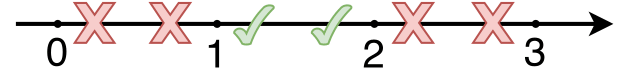
\includegraphics[width=0.55\textwidth]{2/theory/Fig1.png}
    \caption{1D dataset}
    \label{a}
    \end{figure}}
%     \item {[2 points] In the same dataset, can you propose a 2-D transformation that makes the points linearly separable?}

    \item { [2 points] 
    \enfr{
    Consider the following 2-D dataset (Figure \ref{b}). Can you propose a transformation into 1D that will make the data linearly separable? 
    }{
    Soit les données 2-D suivantes (Figure \ref{b}). Pouvez-vous proposer une transformation 1-D qui rend les points linéairement séparables?
    }
    \begin{figure}[h]
    \centerline{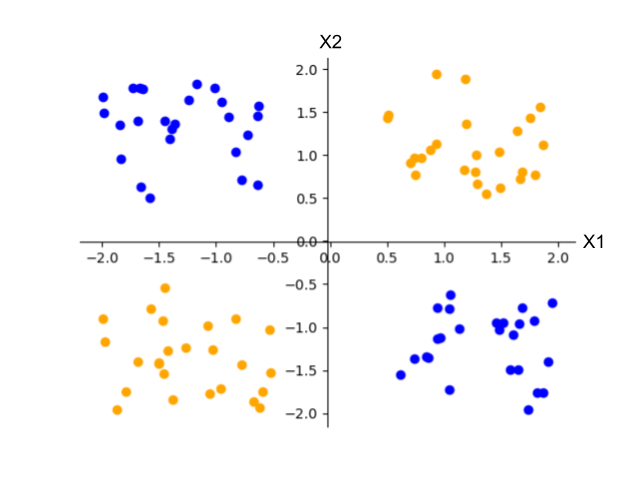
\includegraphics[scale=0.4]{2/theory/Fig2.png}}
    \caption{2D dataset}
    \label{b}
    \end{figure}}

    \item { [4 points] 
    \enfr{
    Using ideas from the above two datasets, can you suggest a transformation of the following dataset (as shown in Figure \ref{12}) that makes it linearly separable? If `\textit{yes}', also provide the kernel corresponding to the feature map you proposed. 
    }{
    En utilisant les idées que vous avez utilisées pour les deux questions précédentes, pouvez-vous proposer une transformation 2-D des données suivantes (Figure \ref{12}) qui les rendent linéairement séparables? Si votre réponse est `\textit{oui}', donnez l'expression du noyau qui correspond à la transformation proposée.
    }
    \begin{figure}[ht]
    \centering
    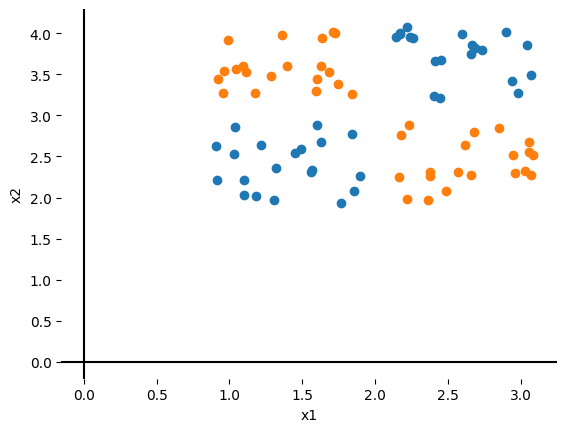
\includegraphics[scale=0.5]{2/theory/Fig3.png}
    \caption{Another 2D dataset}
    \label{12}
    \end{figure}}
    
\end{enumerate} 
}


\end{enumerate}

%%%%%%%%%%%%%%%%%%%%%%%%%%%%%%%%%%%%%%%%%%%%%%%%%%%%%%%%%%%%%
% \section{Practical Part (7 pts) \footnotesize{\textit{Partie pratique}}}

% \input{homework1/practical-part.tex}




\end{document}